\documentclass{standalone}
    \usepackage{tikz}
    \usepackage{pgfplots}
    \usetikzlibrary{calc}
    \usetikzlibrary{patterns}
\mathversion{bold}
% defining the new dimensions and parameters
\newlength{\hatchspread}
\newlength{\hatchthickness}
\newlength{\hatchshift}
\newcommand{\hatchcolor}{}
% declaring the keys in tikz
\tikzset{hatchspread/.code={\setlength{\hatchspread}{#1}},
         hatchthickness/.code={\setlength{\hatchthickness}{#1}},
         hatchshift/.code={\setlength{\hatchshift}{#1}},% must be >= 0
         hatchcolor/.code={\renewcommand{\hatchcolor}{#1}}}
% setting the default values
\tikzset{hatchspread=3pt,
         hatchthickness=0.4pt,
         hatchshift=0pt,% must be >= 0
         hatchcolor=black}
% declaring the pattern
\pgfdeclarepatternformonly[\hatchspread,\hatchthickness,\hatchshift,\hatchcolor]% variables
   {custom north west lines}% name
   {\pgfqpoint{\dimexpr-2\hatchthickness}{\dimexpr-2\hatchthickness}}% lower left corner
   {\pgfqpoint{\dimexpr\hatchspread+2\hatchthickness}{\dimexpr\hatchspread+2\hatchthickness}}% upper right corner
   {\pgfqpoint{\dimexpr\hatchspread}{\dimexpr\hatchspread}}% tile size
   {% shape description
    \pgfsetlinewidth{\hatchthickness}
    \pgfpathmoveto{\pgfqpoint{0pt}{\dimexpr\hatchspread+\hatchshift}}
    \pgfpathlineto{\pgfqpoint{\dimexpr\hatchspread+0.15pt+\hatchshift}{-0.15pt}}
    \ifdim \hatchshift > 0pt
      \pgfpathmoveto{\pgfqpoint{0pt}{\hatchshift}}
      \pgfpathlineto{\pgfqpoint{\dimexpr0.15pt+\hatchshift}{-0.15pt}}
    \fi
    \pgfsetstrokecolor{\hatchcolor}
%    \pgfsetdash{{1pt}{1pt}}{0pt}% dashing cannot work correctly in all situation this way
    \pgfusepath{stroke}
   }

\begin{document}
\Large
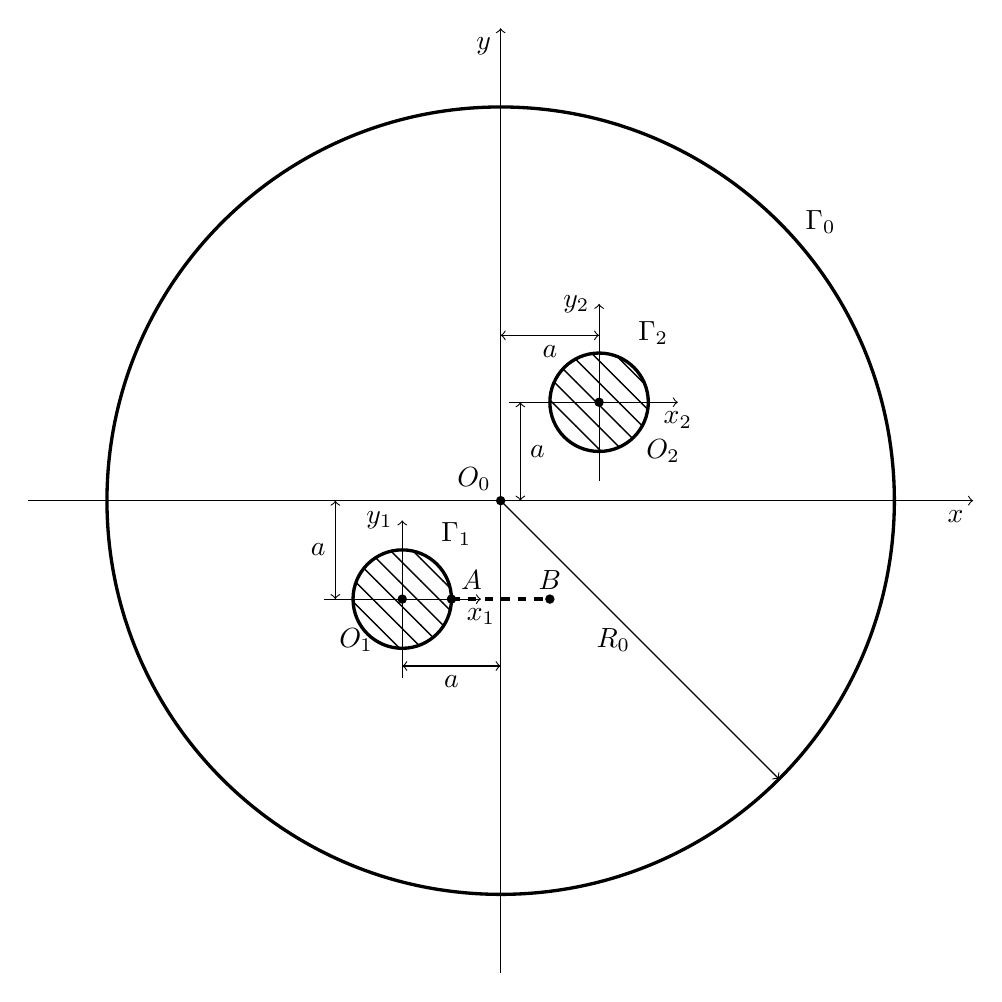
\begin{tikzpicture}[scale=5]
\coordinate (O) at (0,0);
\coordinate (O1) at (-0.25,-0.25);
\coordinate (O2) at (0.25,0.25);
\coordinate (A) at (-0.125,-0.25);
\coordinate (B) at (0.125,-0.25);

\draw[very thick] let \n{radius} = {1.0} in (O) circle (\n{radius});
\draw[->] ($ (-1.2,0) $) -- ($ (1.2,0) $) node[below left] {$x$};
\draw[->] ($ (0,-1.2) $) -- ($ (0,1.2) $) node[below left] {$y$};
\draw[very thick] (O1) circle (0.125);
%\fill[pattern = north east lines] (O1) circle(0.125);
\fill[pattern=custom north west lines,hatchspread=8pt,hatchthickness=0.5pt,hatchcolor=black] (O1) circle(0.125);
\node[below left] at (-0.3,-0.3) {$O_1$};
\node[below left] at (-0.05,-0.03) {$\Gamma_1$};
\draw[->] (-0.45,-0.25) -- (-0.05,-0.25) node[below] {$x_1$};
\draw[->] (-0.25,-0.45) -- (-0.25,-0.05) node[left] {$y_1$};
\draw[very thick] (O2) circle (0.125);
%\fill[pattern = north east lines] (O2) circle(0.125);
\fill[pattern=custom north west lines,hatchspread=8pt,hatchthickness=0.5pt,hatchcolor=black] (O2) circle(0.125);
\node[below left] at (0.48,0.18) {$O_2$};
\node[below left] at (0.45,0.48) {$\Gamma_2$};
\draw[->] (0.02,0.25) -- (0.45,0.25) node[below] {$x_2$};
\draw[->] (0.25,0.05) -- (0.25,0.5) node[left] {$y_2$};

\fill (O) circle(0.012) node[above left] {$O_0$};
\fill (O1) circle(0.012);
\fill (O2) circle(0.012);
\fill (A) circle(0.012);
\fill (B) circle(0.012);

\node[above right] at (A) {$A$};
\node[above] at (B) {$B$};
\draw[very thick,dashed] (A) -- (B);

\draw[<->] (-0.42,-0.25) -- (-0.42,0);
\node[left] at (-0.42,-0.125) {$a$};

\draw[<->] (-0.25,-0.42) -- (0,-0.42);
\draw[<->] (0.25,0.42) -- (0,0.42);
\draw[<->] (0.05,0) -- (0.05,0.25);
\node[below] at (-0.125,-0.42) {$a$};
\node[below] at (0.125,0.42) {$a$};
\node[right] at (0.05,0.125) {$a$};

\draw[->] (O) -- (0.707107,-0.707107);
\node[left] at (0.353553,-0.353553) {$R_0$};
\node[right] at (0.75,0.707107) {$\Gamma_0$};

\end{tikzpicture}
\end{document}

%%% Local Variables: 
%%% mode: latex
%%% TeX-master: t
%%% End: 
